%%%%%%%%%%%%%%%%%%%%%%%%%%%%%%%%%%%%%%%%%%%%%%%%%%%
%% LaTeX book template                           %%
%% Author:  Amber Jain (http://amberj.devio.us/) %%
%% License: ISC license                          %%
%%%%%%%%%%%%%%%%%%%%%%%%%%%%%%%%%%%%%%%%%%%%%%%%%%%

\documentclass[a4paper,11pt, oneside]{book}
\usepackage[T1]{fontenc}
\usepackage[utf8]{inputenc}
\usepackage{lmodern}
%%%%%%%%%%%%%%%%%%%%%%%%%%%%%%%%%%%%%%%%%%%%%%%%%%%%%%%%%
% Source: http://en.wikibooks.org/wiki/LaTeX/Hyperlinks %
%%%%%%%%%%%%%%%%%%%%%%%%%%%%%%%%%%%%%%%%%%%%%%%%%%%%%%%%%
\usepackage{hyperref}
\usepackage{graphicx}
\usepackage[english]{babel}
\usepackage{verbatimbox}
\usepackage{graphicx}
\graphicspath{ {diagrams/}{schedule/}{user-interface/} }
\usepackage{float}
\usepackage{pdfpages}

%%%%%%%%%%%%%%%%%%%%%%%%%%%%%%%%%%%%%%%%%%%%%%%%%%%%%%%%%%%%%%%%%%%%%%%%%%%%%%%%
% 'dedication' environment: To add a dedication paragraph at the start of book %
% Source: http://www.tug.org/pipermail/texhax/2010-June/015184.html            %
%%%%%%%%%%%%%%%%%%%%%%%%%%%%%%%%%%%%%%%%%%%%%%%%%%%%%%%%%%%%%%%%%%%%%%%%%%%%%%%%
\newenvironment{dedication}
{
   \cleardoublepage
   \thispagestyle{empty}
   \vspace*{\stretch{1}}
   \hfill\begin{minipage}[t]{0.66\textwidth}
   \raggedright
}
{
   \end{minipage}
   \vspace*{\stretch{3}}
   \clearpage
}

%%%%%%%%%%%%%%%%%%%%%%%%%%%%%%%%%%%%%%%%%%%%%%%%
% Chapter quote at the start of chapter        %
% Source: http://tex.stackexchange.com/a/53380 %
%%%%%%%%%%%%%%%%%%%%%%%%%%%%%%%%%%%%%%%%%%%%%%%%
\makeatletter
\renewcommand{\@chapapp}{}% Not necessary...
\newenvironment{chapquote}[2][2em]
  {\setlength{\@tempdima}{#1}%
   \def\chapquote@author{#2}%
   \parshape 1 \@tempdima \dimexpr\textwidth-2\@tempdima\relax%
   \itshape}
  {\par\normalfont\hfill--\ \chapquote@author\hspace*{\@tempdima}\par\bigskip}
\makeatother

%%%%%%%%%%%%%%%%%%%%%%%%%%%%%%%%%%%%%%%%%%%%%%%%%%%
% First page of book which contains 'stuff' like: %
%  - Book title, subtitle                         %
%  - Book author name                             %
%%%%%%%%%%%%%%%%%%%%%%%%%%%%%%%%%%%%%%%%%%%%%%%%%%%

% Book's title and subtitle
\title{\Huge \textbf{Road Surface Estimator} \\ \huge A Project Proposal}
% Author
\author{\textsc{Thanakrit Lee}}


\begin{document}

\frontmatter
\maketitle

%%%%%%%%%%%%%%%%%%%%%%%%%%%%%%%%%%%%%%%%%%%%%%%%%%%%%%%%%%%%%%%%%%%%%%%%
% Auto-generated table of contents, list of figures and list of tables %
%%%%%%%%%%%%%%%%%%%%%%%%%%%%%%%%%%%%%%%%%%%%%%%%%%%%%%%%%%%%%%%%%%%%%%%%
\tableofcontents

\mainmatter

%%%%%%%%%%%%%%%%%%%%%%%%%%%%%%%%%%%%%%%%%%%%%%%%%%%%%%%%%%%%%%%%%%%%%%%%

\chapter{Introduction}

Re-surfacing roads requires the knowledge of the surface area of roads to resurface.
Getting the surface area of roads can be made more efficient using aerial/satellite views technology, where the surface area can be calculated. The efficiency of having a total estimated surface area of roads to resurface allows road surface materials to be prepared in a more precise manner, reducing materials wastes and thus reducing total road resurfacing costs.


This document propose a web application that allows user to designate point on a map for a total estimated surface area of roads in the square kilometre ($km^2$). The web application will be implemented with Google Maps, which allows for user to map interactivity, and for getting data requires for the surface area calculation.

%%%%%%%%%%%%%%%%%%%%%%%%%%%%%%%%%%%%%%%%%%%%%%%%%%%%%%%%%%%%%%%%%%%%%%%%

\chapter{Project Requirements}

\section{Functional Requirements}

\begin{itemize}
	\item The application is able to display a graphical map.
	\item The application allow user to interact with the map e.g. click on the map, drag and move around on the map, zoom in and zoom out, change map styling (roadmap and satellite view), add marker, move marker by dragging it, click on marker to show marker info.
	\item The application allow user to mark the centre point of the square kilometre area on the interactive map.
	\item The application allow user to input longitude and latitude coordinates.
	\item The application is able to display the user input coordinates on the interactive map.
	\item The application is able to calculate the surface area of the road in the selected square kilometre ($km^2$).
	\item The application is able to display the calculated road surface area.
\end{itemize}

\section{Non-Functional Requirements}
\begin{itemize}
	\item The application's graphical user interface is easy to navigate.
	\item The application is doesn't take long to process the surface area calculation, i.e. low response time.
	\item The application is responsive.
	\item The application is able to be use on mobile devices.
	\item The application provides an easy to understand tutorial on how to use the application.
	\item The application is hosted on the web, and user can access via the internet.
\end{itemize}


%%%%%%%%%%%%%%%%%%%%%%%%%%%%%%%%%%%%%%%%%%%%%%%%%%%%%%%%%%%%%%%%%%%%%%%%

\chapter{Project Plan}

\section{Overview}
The objective of the project is to develop a web application that allows user to select a square kilometre area on the interactive map, calculate the total estimated surface area of roads in the area, and display the result.

A constraint for the project is that this project is done as part of a contract for a local council in Victoria, Melbourne, Australia. This means that the roads to resurface must be the correct category of roads classified by the local council (i.e. the declared roads being free ways, arterial roads and some non-arterial state roads)\cite{WEBSITE:5}

\section{Risk Analysis}

\addvbuffer[12pt 8pt]{
\begin{tabular}{ |p{1cm}||p{6cm}|p{6cm}| }
	\hline
	\multicolumn{3}{|c|}{\textbf{Risk List}} \\
	\hline
	\textbf{ID} & \textbf{Risk} & \textbf{Trigger} \\
	\hline
	R0 	& 	Project scope creep 	&	 Project scope wasn't defined properly. \\
	\hline
	R1	&	Software libraries, modules or frameworks changes and is now incompatible with the project	&  The software developers making changes to the software. \\
	\hline
	R2	&	Working computer breaks		&	Dropping the computer, spilling water on it. \\
	\hline
	R3	&	Project going over schedule		&	Improper time management of the project, not regularly updating and checking on the project schedule Gantt Chart.s \\
	\hline
\end{tabular}}


\addvbuffer[12pt 8pt]{
\begin{tabular}{ |p{1cm}||p{6cm}|p{6cm}| }
	\hline
	\multicolumn{3}{|c|}{\textbf{Risk List}} \\
	\hline
	\textbf{ID} & \textbf{Probability (low/medium/high)} & \textbf{Impact (low/medium/high)} \\
	\hline
	R0 & low & high \\
	\hline
	R1 & low & medium \\
	\hline
	R2 & low & high \\
	\hline
	R3 & medium & high \\
	\hline
\end{tabular}}

\addvbuffer[12pt 8pt]{
\begin{tabular}{ |p{1cm}||p{12.43cm}| }
	\hline
	\multicolumn{2}{|c|}{\textbf{Risk List}} \\
	\hline
	\textbf{ID} & \textbf{Mitigation Plan} \\
	\hline
	R0 & Make sure to get most (if not all) the project requirements from the project stakeholders. If a compulsory requirement is added, make it a priority over lower priority requirements. \\
	\hline
	R1 & Use versioning tool to keep track of the version of the libaries the project is using. \\
	\hline
	R2 & Take good care of the computer. Backup the project code regularly. Use Git remote repository (such as GitHub\cite{WEBSITE:8}) to backup the project and regularly make commits and push to the remote repository. \\
	\hline
	R3 & Regularly check the project schedule to see where the project progress is at and compare it to the current time to see if the project is behind, ahead or on schedule. Make a commitment to at keep the project on schedule. If the project is behind schedule then work over time to catch up to the project schedule time line.  \\
	\hline
\end{tabular}}	

\section{Resource Requirements}
\begin{itemize}
	\item Computer for developing the project.
	\item Internet access to download and use libraries the project depends on, and to access the libraries documentation.
	\item Angular 5.2.0\cite{WEBSITE:1}, a front end framework use for creating a good user interface and implementing business logic.
	\item Node.js 8.9.4\cite{WEBSITE:2}, a JavaScript runtime for use with Express.js to create a server API and implement the back end of the web application.
	\item Express.js 4.16.3\cite{WEBSITE:4}, for creating the API for communication between client and server.
	\item MDBootstrap 5.2.3\cite{WEBSITE:7}, use the CSS framework for faster development of the app.
	\item AGM 1.0.0\cite{WEBSITE:6}, a wrapper of Google Maps JavaScript API for Angular 2+.
\end{itemize}

\section{Schedule}

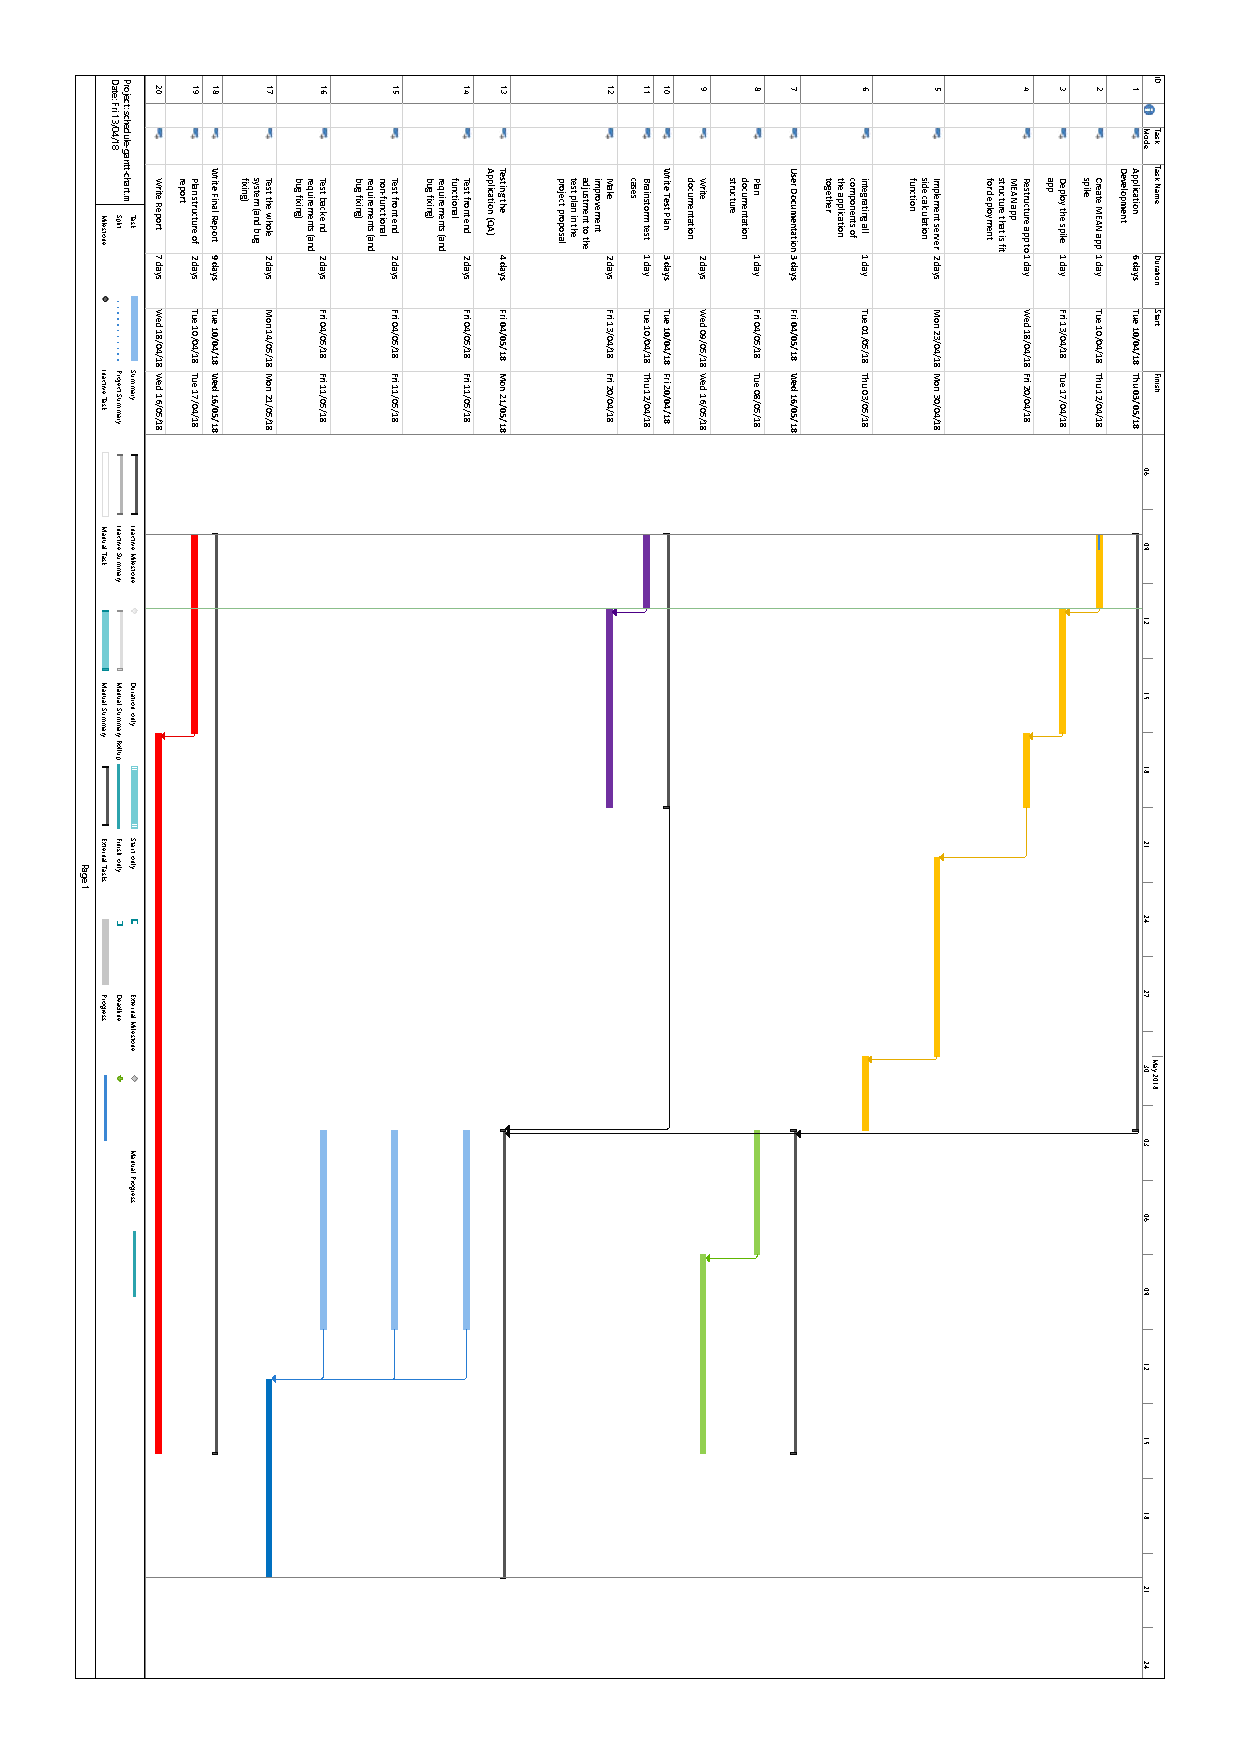
\includepdf[pages={1}]{schedule/schedule-gantt-chart-rotated.pdf}

%%%%%%%%%%%%%%%%%%%%%%%%%%%%%%%%%%%%%%%%%%%%%%%%%%%%%%%%%%%%%%%%%%%%%%%%

\chapter{External Design}


\section{User Interface}

The user interface of the web application will be responsive. It can be view on both the computer web browser and the mobile phone web browser. 

Figure (4.1, 4.2) shows the web application user interface on the computer web browser. The "Calculate Road Surface Area" page is for using the main functionality of the application (getting the surface area). It includes a Google Maps for user to interact with, the user can zoom, move around, add centred marker (the map is centred to the marker when it's added) on the map, move the marker around by clicking on it and dragging it, and click on a marker to get more information about the marker (coordinates).

Figure (4.3, 4.4, 4.5, 4.6) shows the web application user interface on the mobile phone web browser. Depending on how small the size of the screen of the mobile device is the navigation bar at the top of the page will compress and becomes a navigation bar that drop downs the navigation links. The suer can drop down the navigation links by tapping on the "burger" icon on the right side of the navigation bar.

User can choose to add marker by tapping on the interactive Google Maps or by entering the latitude and longitude coordinates in the input field. The input fields is reveal and hidden with the use of the "USE COORDINATES INSTEAD" button.

This user interface mockup is not how the finalise version of the application will look like. Changes to colour scheme and layout of components are likely to change to increase the application usability, e.g. user experience, making the application easier to use, pleasant to look at and use etc.

\begin{figure}[H]
	\begin{minipage}[b]{0.4\textwidth}
		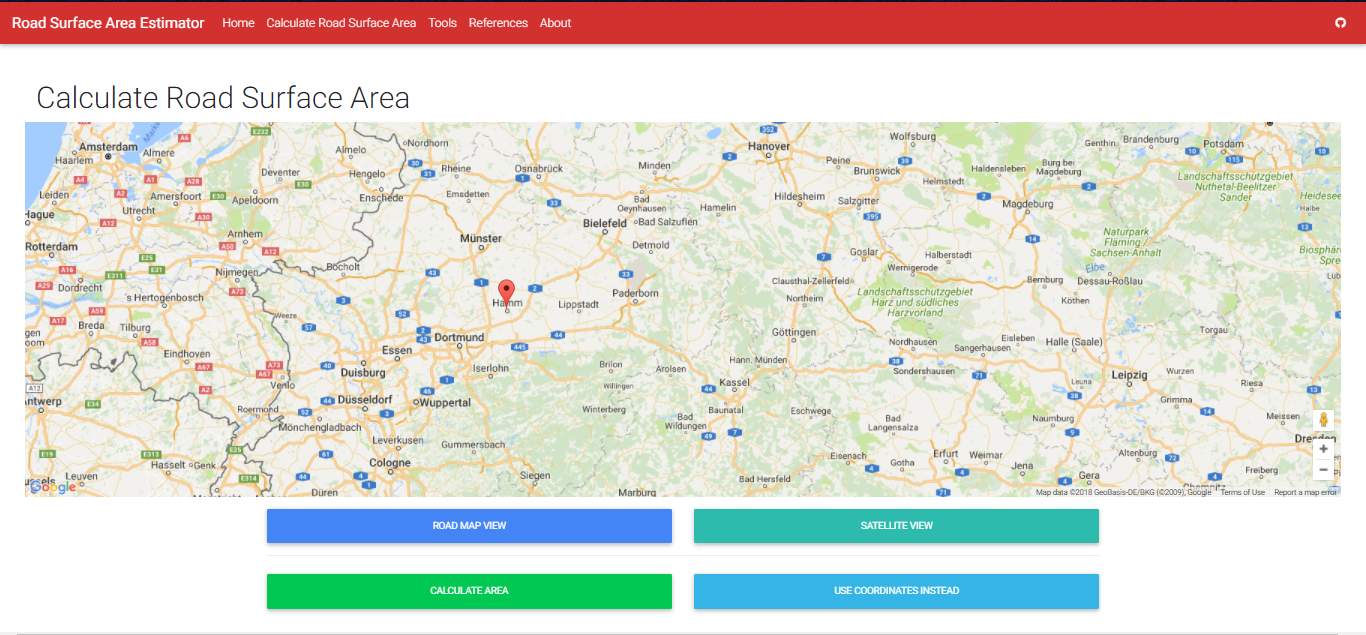
\includegraphics[scale=0.4]{web-calculate-area-0}
		\caption{Computer web browser view 1}
	\end{minipage}
\end{figure}

\begin{figure}[H]
	\begin{minipage}[b]{0.4\textwidth}
		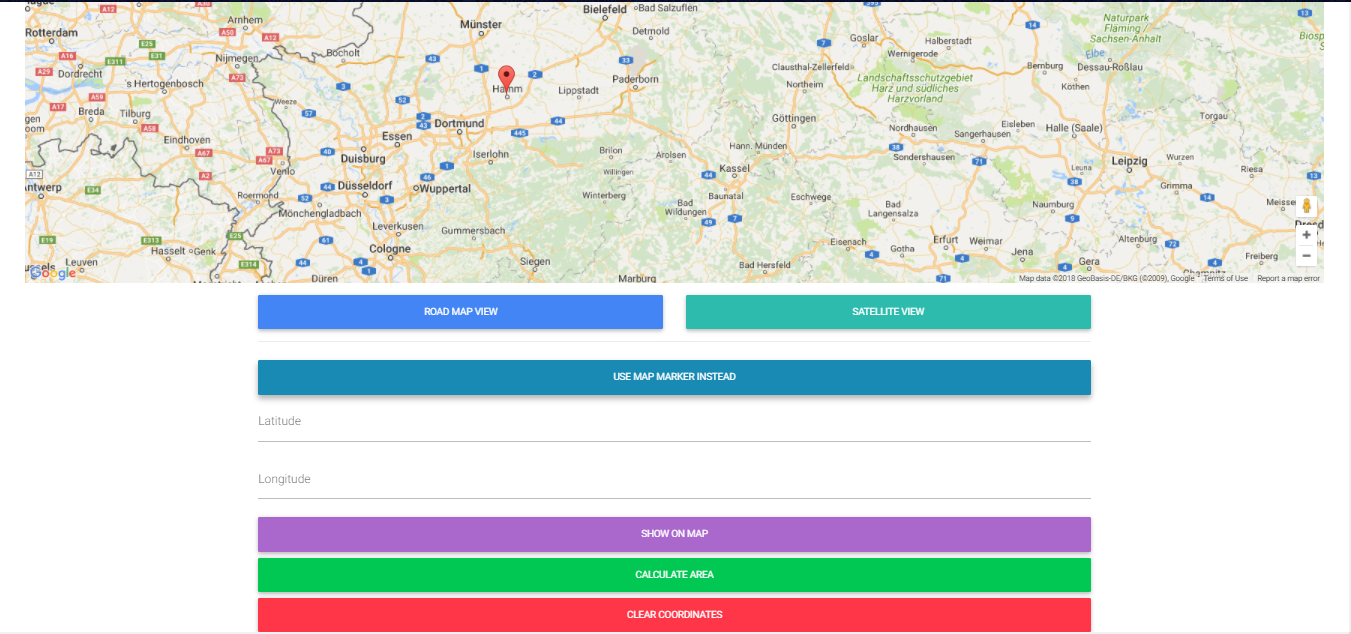
\includegraphics[scale=0.4]{web-calculate-area-1}
		\caption{Computer web browser view 2}
	\end{minipage}
\end{figure}

\begin{figure}[H]
	\centering
	\begin{minipage}[b]{0.4\textwidth}
		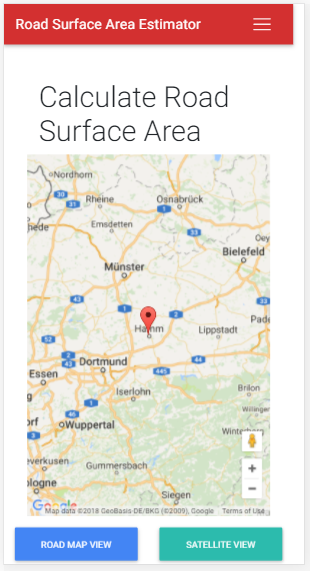
\includegraphics[width=\textwidth]{mobile-calculate-area-0}
		\caption{Mobile phone view 1}
	\end{minipage}
	\hfill
	\begin{minipage}[b]{0.4\textwidth}
		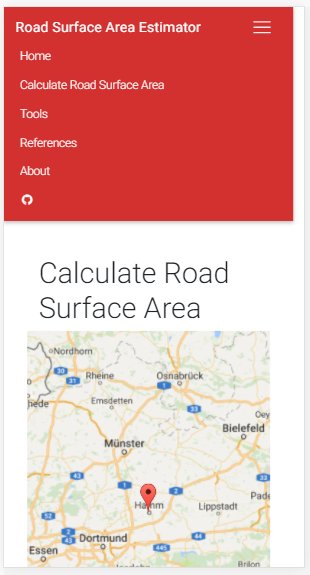
\includegraphics[width=\textwidth]{mobile-calculate-area-1}
		\caption{Mobile phone view 2}
	\end{minipage}
\end{figure}
\begin{figure}[H]
	\centering
	\begin{minipage}[b]{0.4\textwidth}
		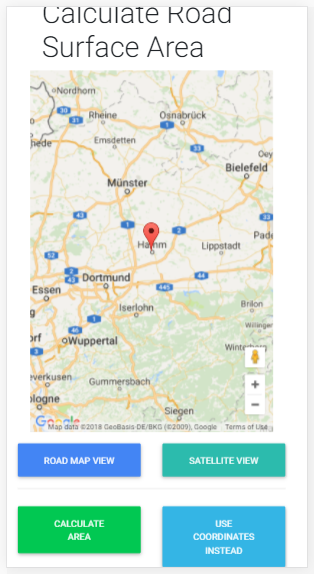
\includegraphics[width=\textwidth]{mobile-calculate-area-2}
		\caption{Mobile phone view 3}
	\end{minipage}
	\hfill
	\begin{minipage}[b]{0.4\textwidth}
		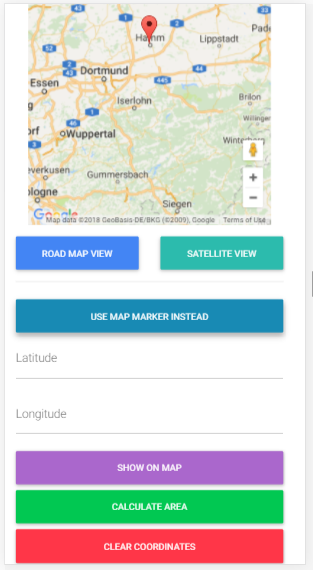
\includegraphics[width=\textwidth]{mobile-calculate-area-3}
		\caption{Mobile phone view 4}
	\end{minipage}
\end{figure}

\section{Performance}
Time complexity of the server processing the image and making the surface area calculation is $O(n)$, where $n$ is the number of pixels in the map image. It is of that time complexity because the server will run through all pixels in the image array once and collects "road pixels", then it will add all the surface area of the collected "road-pixels" together to get the estimated total road surface area.


%%%%%%%%%%%%%%%%%%%%%%%%%%%%%%%%%%%%%%%%%%%%%%%%%%%%%%%%%%%%%%%%%%%%%%%%

\chapter{Internal Design}
The web application will have a client-side and server-side. Angular 5 is use as the front-end client-side and Node JS Express is use as the back-end server-side. The client and server will communicates with each other through HTTP. A server is implemented in this web application so that it is properly structured and follow the separation of concerns principle. The front-end take cares of the business logic (displaying data, taking user inputs) while the back-end take cares of the calculation and processing of data.

\begin{figure}[H]
	\begin{minipage}[b]{0.4\textwidth}
		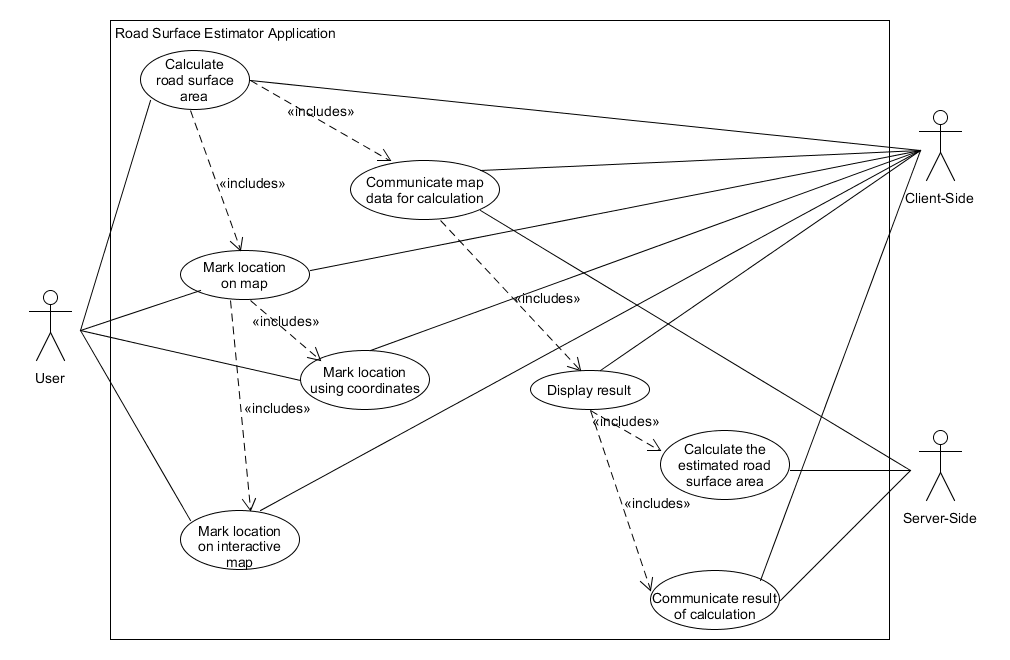
\includegraphics[scale=0.4]{use-case}
		\caption{Use Case diagram}
	\end{minipage}
\end{figure}

\begin{figure}[H]
	\begin{minipage}[b]{0.4\textwidth}
		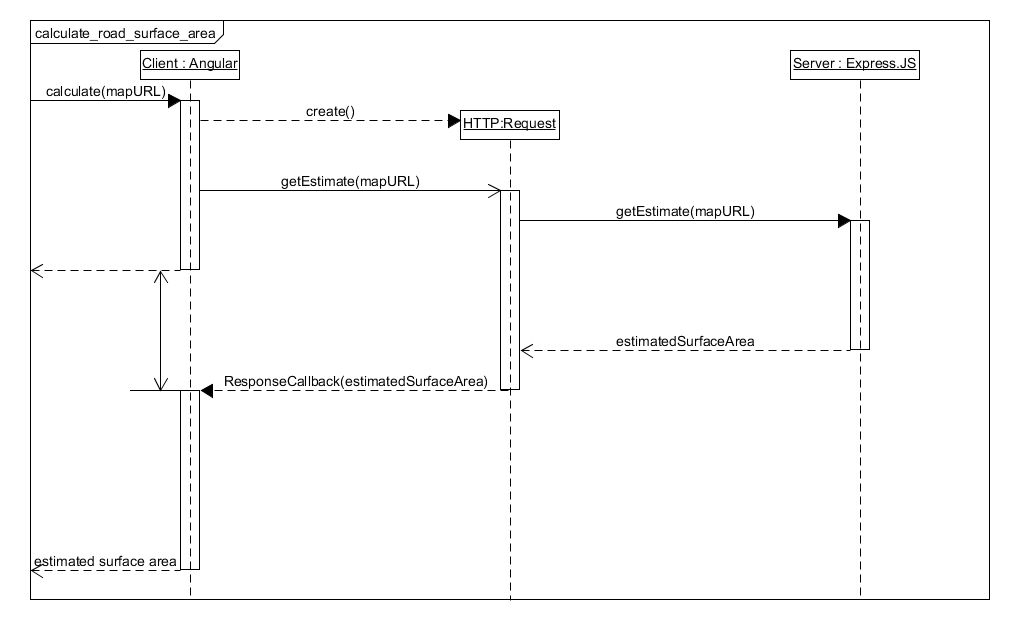
\includegraphics[scale=0.4]{squence-diagram}
		\caption{Sequence diagram}
	\end{minipage}
\end{figure}

%%%%%%%%%%%%%%%%%%%%%%%%%%%%%%%%%%%%%%%%%%%%%%%%%%%%%%%%%%%%%%%%%%%%%%%%

\chapter{Software Architecture}
The web application will use the Angular 5 web framework to implement the front-end client-side of the application. The back-end server-side will be implemented using Node JS Express, and the communications between the server and the client will be done through HTTP REST. Using the Google Maps API, the client creates a map static image URL and pass it (through HTTP) to the server for processing. The server will the process the image and calculate the total surface area of roads in the map, and response the result back to the client.

\begin{figure}[H]
	\begin{minipage}[b]{0.4\textwidth}
		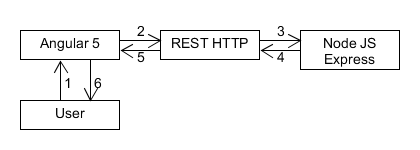
\includegraphics[scale=0.4]{software-architecture}
		\caption{Software Architecture diagram}
	\end{minipage}
\end{figure}

%%%%%%%%%%%%%%%%%%%%%%%%%%%%%%%%%%%%%%%%%%%%%%%%%%%%%%%%%%%%%%%%%%%%%%%%

\chapter{Test Plan}

\section{Test Coverage}

\addvbuffer[12pt 8pt]{
	\begin{tabular}{ |p{1cm}||p{6cm}|p{6cm}| }
		\hline
		\multicolumn{3}{|c|}{\textbf{Test Coverage List}} \\
		\hline
		\textbf{ID} & \textbf{Requirement} & \textbf{Product Life Stage To Verify At} \\
		\hline
		Re0 & Display graphical map & Development \\
		\hline
		Re1 & Have user-to-map interaction & Development \\
		\hline
		Re2 & Have coordinates user input & Development \\
		\hline
		Re3 & Turn user input coordinates into marker on the map & Development \\
		\hline
		Re4 & Calculate estimated total surface area of roads in user selected $km^2$ on the map & Development \\
		\hline
		Re5 & Display surface area result & Development \\
		\hline
		Re6 & Doesn't take "long" to do the surface area calculation & Testing \\
		\hline
		Re7 & Web design is responsive & Testing \\
		\hline
		Re8 & Can be use on mobile device & Testing \\
		\hline
		Re9 & Provides a easy to understand tutorial & Testing \\
		\hline
		Re10 & Can access the application on the internet & Testing \\
		\hline
\end{tabular}}

\section{Test Methods}

\addvbuffer[12pt 8pt]{
	\begin{tabular}{ |p{1cm}||p{12.43cm}| }
		\hline
		\multicolumn{2}{|c|}{\textbf{Test Methods List}} \\
		\hline
		\textbf{ID} & \textbf{Testing Implementation Method} \\
		\hline
		Re0 & Unit Testing \\
		\hline
		Re1 & Integration Testing \\
		\hline
		Re2 & Unit Testing \\
		\hline
		Re3 & Integration Testing \\
		\hline
		Re4 & Integration Testing \\
		\hline
		Re5 & Unit Testing \\
		\hline
		Re6 & Performance Testing \\
		\hline
		Re7 & Usability Testing \\
		\hline
		Re8 & System Testing \\
		\hline
		Re9 & Usability Testing \\
		\hline
		Re10 & System Testing \\
		\hline
\end{tabular}}

\section{Sample Test Cases}

\addvbuffer[12pt 8pt]{
	\begin{tabular}{ |p{1cm}||p{12.43cm}| }
		\hline
		\multicolumn{2}{|c|}{\textbf{Test Sample Cases List}} \\
		\hline
		\textbf{ID} & \textbf{How the data will be collected} \\
		\hline
		Re0 & By checking that the web application displays a graphical map (Google Maps). \\
		\hline
		Re1 & Interact with the map on the web application page. Interaction includes scrolling to zoom in and out, dragging to move around the map, clicking on the map to add a marker and centre the map on the added marker, change map type and style, dragging a marker, clicking on a marker to show more info. \\
		\hline
		Re2 & Check that the app page has input options for longitude and latitude coordinates. \\
		\hline
		Re3 & Click on the "show on map" button to test the functionality. Check that a new marker is added on the map. Check that the coordinatse of the new marker is the same as the user input coordinates by clicking on the marker to show the marker info which includes its coordinates. \\
		\hline
		Re4 & Check that the map area to calculate is 1 $km^2$. Check that the result is a correct estimate. \\
		\hline
		Re5 & Check the app page to see that a result is shown there. \\
		\hline
		Re6 & Check that the app doesn't take more than 5 seconds to calculate and return the result, by timing the calculate function. \\
		\hline
		Re7 & Change the size of the web browser on the laptop to see if web app is responsive. Change the size of the mobile device in chrome developer tools\cite{WEBSITE:3} to see if web app is also responsive to different phone screen size. \\
		\hline
		Re8 & Use chrome developer tools and change to mobile view and check that the web app works on the mobile devices. Using a real physical phone, on the phone web browser go to the web app address and check that the app works on the phone. \\
		\hline
		Re9 & Get a user to use the application and ask for inputs, comments, and opinions afterwards. \\
		\hline
		Re10 & On both a computer and mobile phone, use the web browser and go to the address of the web application and test that the application works by checking all functionalities. \\
		\hline
		
\end{tabular}}
%%%%%%%%%%%%%%%%%%%%%%%%%%%%%%%%%%%%%%%%%%%%%%%%%%%%%%%%%%%%%%%%%%%%%%%%

\chapter{References}
\bibliography{reference/reference}
\bibliographystyle{apalike}

%%%%%%%%%%%%%%%%%%%%%%%%%%%%%%%%%%%%%%%%%%%%%%%%%%%%%%%%%%%%%%%%%%%%%%%%

\end{document}